\documentclass[a4paper,11pt,fleqn]{article}%fleqn pour aligner les equations à gauche
\usepackage{/home/rweye/Documents/Overleaf/Styles/Exercice}


\newcommand{\chnum}{Chapitre 6}
\newcommand{\chtitle}{Equilibres chimiques}
\newcommand{\dtype}{Exercices}
  
  
\begin{document}
\maketitle

\begin{multicols}{2}
\section{Calcul d'un quotient de réaction}
Les ions iodure \ce{I^{-}(aq)}, en contact avec les ions peroxodisulfate \ce{S2O8^{2-}(aq)}, subissant une oxydation lente. On s'intéresse au mélange de \num{100} \unit{\milli \liter} d'une solution de peroxodisulfate d'ammonium (\ce{2 NH4^{+}(aq)} ;\ce{S2O8^{2-}(aq)}) de concentration $c_1$ = \num{0,10} \unit{\mole \per \liter} avec \num{100} \unit{\milli \liter} de solution d'iodure de potassium (\ce{K^{+}(aq)} ; \ce{I^{-}(aq)}) de concentration $c_2$ = \num{0,20} \unit{\mole \per \liter}.
\begin{enumerate}
	\item Établir l'équation de la réaction à partir des couples fournis.
	\item Exprimer le quotient de réaction $Q_r$.
	\item Calculer sa valeur à l'état initial.
\end{enumerate}
La constante d'équilibre de cette réaction est égale à $K$ = \num{2e46}.
\begin{enumerate}
\setcounter{enumi}{3}
	\item Conclure quant au caractère total ou non de la réaction.
\end{enumerate}
\textbf{Données :}\\
Couples d'oxydoréduction : \ce{I2(aq) / I-(aq)} et \ce{S2O8^{2-}(aq) / SO4^{2-}(aq)}

\section{Calcul de la constante d'équilibre}
L'acide ascorbique \ce{C6H8O6}, plus connu sous le nom de vitamine C, réagit avec l'eau selon l'équation : \\
\ce{C6H8O6(aq) +H_2O(l) <=> C6H7O6-(aq) + H3O+(aq)}\\
À l'équilibre, les concentrations sont les suivantes :
\begin{itemize*}
	\item $[\ce{C6H8O6}]$ = \num{2,6e-1} \unit{\mole \per \liter}
	\item $[\ce{C6H7O6^{-}}]$ = \num{3,1e-3} \unit{\mole \per \liter}
	\item $[\ce{H3O^{+}}]$ = \num{6,7e-3} \unit{\mole \per \liter}
\end{itemize*}
Calculer la constante d'équilibre $K$ de cette réaction.

\section{Accident domestique}
L'eau de Javel est une solution aqueuse contenant des ions chlorure \ce{Cl^{-}(aq)}, des ions hypochlorite \ce{ClO^{-}(aq)} et des ions sodium \ce{Na^{+}(aq)}. Mélangé à une solution acide contenant des ions oxonium \ce{H3O^{+}(aq)}, ce produit ménager peut réagir selon l'équation suivante :\\
\ce{ClO^{-}(aq) + Cl^{-}(aq) + 2 H3O^{+}(aq) <=> Cl2(aq) + 2 H2O(l)}
\begin{enumerate}
	\item Exprimer le quotient de réaction $Q_r$
	\item Compte tenu de la constante d'équilibre fournie, et en supposant que tout le dichlore \ce{Cl2(aq)} formé pour \num{2,0} \unit{\gram} d'ions hypochlorite \ce{ClO-(aq)} réagissant avec les ions oxonium \ce{H3O+(aq)} et chlorure \ce{Cl-(aq)} en excès.
	\item Le dichlore \ce{Cl2(aq)} en solution passe rapidement dans l'air, ce qui diminue sa concentration en solution. En déduire le sens d'évolution de la réaction.
	\item Expliquer le danger à nettoyer ses toilettes en y versant de l'acide chlorhydrique puis de l'eau de Javel.
\end{enumerate}
\textbf{Données :}\\
\begin{itemize}
	\item Volume molaire à \num{20} \unit{\celsius} sous \num{1,013} \unit{\hecto \pascal} : $V_m$ = \num{24} \unit{\liter \per \mole}
	\item Constante d'équilibre : $K$ = \num{3,2e5}
\end{itemize}

\section{Odeur tropicale}
Le méthanoate d'éthyle \ce{C3H6O2} est un ester présentant une odeur de rhum. Il est utilisé dans l'industrie alimentaire pour parfumer des aliments sans avoir à les alcooliser directement avec du rhum. L'acide méthanoïque \ce{HCOOH} et l'éthanol \ce{C2H6O} sont à l'origine de la synthèse de cet ester.
\begin{enumerate}
	\item Écrire l'équation de la synthèse de cet ester et identifier la seconde espèce chimique produite.
\end{enumerate}
Dans un ballon de \num{250} \unit{\milli \liter} sont introduits \num{70} \unit{\milli \liter} d'éthanol de masse volumique $\rho_1$, quatre gouttes de solution d'acide sulfurique concentré \ce{H2SO4(aq)} et quelques grains de pierre ponce. On ajoute \num{45} \unit{\milli \liter} d'acide méthanoïque de masse volumique $\rho_2$. Le mélange est chauffé à reflux jusqu'à obtention de tout l'ester possible. L'état d'équilibre est atteint.
\begin{enumerate}
\setcounter{enumi}{1}
	\item \begin{enumerate}
			\item Préciser le rôle de l'acide sulfurique
			\item Identifier le montage à reflux. Nommer l'autre montage.
	\end{enumerate}
\end{enumerate}
\newpage
\begin{center}
Montage 1 :\\
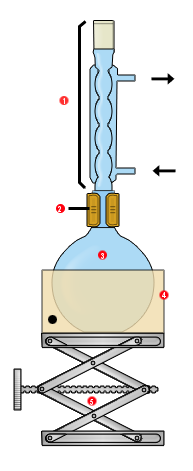
\includegraphics[width=.5\linewidth]{Ressources/TSPE_C7_Exercices_Fig1.png}\\
Montage 2 : \\
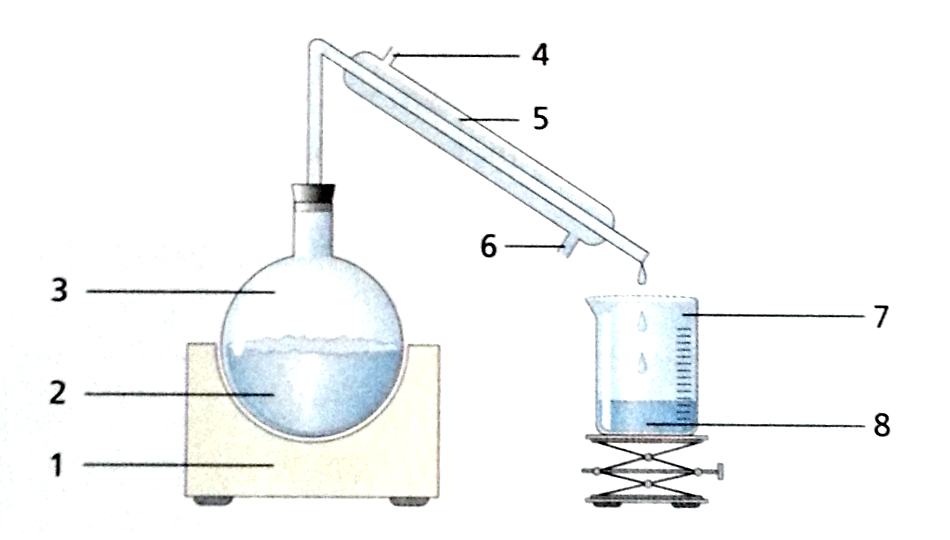
\includegraphics[width=\linewidth]{Ressources/TSPE_C7_Exercices_Fig2.png}
\end{center}
\begin{enumerate}[resume]
	\item \begin{enumerate}
		\item Réaliser le tableau d'avancement de la réaction
		\item Calculer le taux d'avancement final de la réaction.
	\end{enumerate}
\end{enumerate}
\textbf{Données : }
\begin{itemize*}
	\item Masses volumiques : $\rho_1$ = \num{0,789} \unit{\gram \per \milli \liter} et $\rho_2$ = \num{1,22} \unit{\gram \per \milli \liter} 
	\item Quantités de matière à l'état final : $n(\ce{C3H6O2})$ = \num{0,80} \unit{\mole} et $n(\ce{HCOOH})$ = $n(\ce{C2H6O})$ = \num{0,40} \unit{\mole}
	\item Masses molaires : $M(C)$ = \num{12,0} \unit{\gram \per \mole}, $M(H)$ = \num{1,0} \unit{\gram \per \mole} et $M(O)$ = \num{16,0} \unit{\gram \per \mole}
\end{itemize*}

\section{Tension à vide d'une pile}
Une pile alcaline fonctionne à partir des couples \ce{Zn(s)}/\ce{ZnO(s)} à l'anode et \ce{MnO2(s)}/\ce{Mn2O3(s)} à la cathode.

\begin{enumerate}
    \item Rappeler ce qu'est la tension à vide d'une pile.
    \item On place un voltmètre aux bornes de la pile, sa borne COM est reliée à la cathode. La tension à vide de cette pile est de \SI{4,5}{\volt}. En déduire la valeur affichée par le voltmètre.
\end{enumerate}

\section{Vélo électrique}
Une batterie de vélo à assistance électrique a une capacité électrique de \SI{4}{\ampere \hour}. Sur le plat, la batterie débite un courant de \SI{0,5}{\ampere}. En montée, le courant est de \SI{3}{\ampere}.

\begin{enumerate}
    \item Déterminer la durée de fonctionnement de l'assistance électrique sur une route horizontale.
    \item Calculer la durée de fonctionnement de l'assistance pour une route exclusivement en pente ascendante.
\end{enumerate}

\section{Pile cuivre-plomb}
La borne d'entrée d'un voltmètre est reliée à la lame de cuivre \ce{Cu(s)} et la borne COM à la lame de plomb \ce{Pb(s)}.

\begin{figure}[H]
    \centering
    \adjustbox{valign=b}{\subfloat[\textbf{Pile cuivre-plomb}]{
    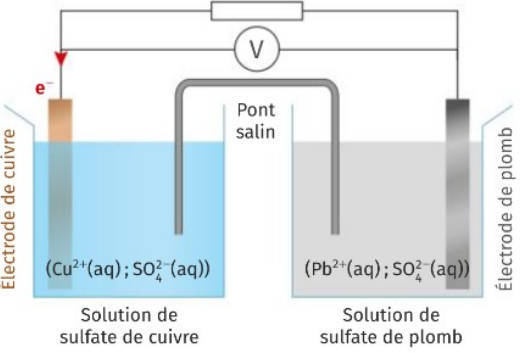
\includegraphics[width=\linewidth]{Ressources/TSPE_C16_Exercices_Fig1.png}}}
\end{figure}

\begin{enumerate}
    \item Déterminer le sens du courant.
    \item Identifier l'anode et la cathode.
    \item À l'aide du schéma, écrire les demi-équations d'oxydoréduction.
    \item En déduire l'équation de fonctionnement de la pile.
\end{enumerate}

\section{Pile nickel-argent}
Une pile nickel argent met en jeu les couples \ce{Ag+(aq)}/\ce{Ag(s)} et \ce{Ni^{2+}(aq)}/\ce{Ni(s)}. Dans la pile, c'est le nickel \ce{Ni(s)} qui s'oxyde.

\begin{enumerate}
    \item Identifier l'anode et la cathode.
    \item Écrire les demi-équations d'oxydoréduction.
    \item En déduire l'équation globale de la réaction de la pile.
    \item Donner la relation entre la capacité électrique, l'intensité du courant et la durée de fonctionnement d'une pile.
    \item Rappeler la relation entre la capacité électrique et la quantité de matière d'électrons échangés.
    \item Calculer la variation de masses de l'anode lorsque la pile a débité un courant continu d'intensité \SI{500}{\milli\ampere} pendant \SI{4,0}{\hour}.
\end{enumerate}

\begin{figure}[H]
    \begin{minipage}{\linewidth}
     \textbf{Données :}
     \begin{itemize}
        \item \textbf{Masses molaires atomiques :}\\
        $M(\ce{Ag})$ = \SI{107,9}{\gram\per\mole} et $M(\ce{Ni})$ = \SI{58,7}{\gram\per\mole}
        \item \textbf{Constante de Faraday :}\\ $F$ = \SI{9,65E4}{\coulomb\per\mole}
    \end{itemize}
    \end{minipage}
\end{figure}

\section{Vitamine C}
L'acide ascorbique \ce{C6H8O6}, dont l'énantiomère L-ascorbique est connu sous le nom de vitamine C, réagit avec l'eau selon l'équation suivante :
$$\ce{C6H8O6(aq) + H2O(l) <=> C6H7O6-(aq) + H3O+(aq)}$$
La constante d'équilibre de la réaction est égale à $K$ = \num{7,9E-5}.

\begin{enumerate}
    \item Préciser la nature de la réaction.
\end{enumerate}
Un comprimé contenant \SI{3,0E-3}{\mole} de vitamine C est dissous sans \SI{200}{\milli\mole} d'eau contenant déjà des ions \ce{C6H7O6-(aq)} à la concentration $[\ce{C6H7O6-}]_i$ = \SI{0,10}{\mole\per\liter}.
\begin{enumerate}[resume]
    \item Avant réaction, déterminer la concentration initiale d'acide ascorbique \ce{C6H8O6(aq)}.
    \item En déduire le sens d'évolution spontanée de cette réaction.
\end{enumerate}
\begin{figure}[H]
    \begin{minipage}{\linewidth}
    \textbf{Donnée :}
    \begin{itemize}
        \item \textbf{pH de la solution avant dissolution du comprimé :} pH = \num{7,8}
    \end{itemize}
    \end{minipage}
\end{figure}

\section{Question de taille}
L'équation de la réaction d'une pile cuivre-zinc est :
$$\ce{Zn(s) + Cu^{2+}(aq) <=> Cu(s) + Zn^{2+}(aq)}$$
La lame de zinc constitue l'anode.
\begin{enumerate}
    \item Écrire les demi-équations associées.
    \item Exprimer la quantité de matière d'électrons transférés.
    \item Calculer la capacité électrique de cette pile.
    \item Les masse de chaque électrode sont doublées. Calculer la nouvelle capacité électrique.
    \item Conclure quant à l'influence de la masse de l'anode et de la cathode.
\end{enumerate}
\begin{figure}[H]
    \begin{minipage}{\linewidth}
    \textbf{Donnée :}
    \begin{itemize}
        \item \textbf{Masses des électrodes :} $m_{anode}$ = \SI{8,0}{\gram} et $m_{cathode}$ = \SI{6,0}{\gram}
        \item \textbf{Constante de Faraday :} $F$ = \SI{9,65E4}{\coulomb\per\mole}
        \item \textbf{Masses molaires :} $M(\ce{Zn})$ = \SI{65,4}{\gram\per\mole} et $M(\ce{Cu})$ = \SI{63,5}{\gram\per\mole}
    \end{itemize}
    \end{minipage}
\end{figure}

\section{Pile citron}
Un moyen simple de réaliser une pile est de planter un trombone recouvert de zinc et une pile recouverte de cuivre dans un citron.//
Une lampe, reliée d'un coté au trombone et de l'autre à la pile, s'allume. Un voltmètre branché à la pile citron affiche \SI{0,84}{\volt}. Sa borne V est du coté du cuivre, la borne COM est reliée au trombone.
\begin{enumerate}
    \item Préciser ce que représente la valeur mesurée.
    \item Déterminer la polarité de la pile au niveau du trombone et de la pièce. Justifier.
\end{enumerate}
Au cours de l'utilisation de la pile, du dihydrogène \ce{H2(g)} se dégage.
\begin{enumerate}[resume]
    \item Écrire les demi-équations d'oxydoréduction ayant lieu à chaque électrode.
    \item En déduire l'équation de réaction globale de la pile citron.
    \item Préciser d'où proviennent les ions \ce{H+(aq)}.
    \item Toujours à partir de citrons, trombones et pièces de cuivre, proposer in dispositif délivrant une tension deux fois plus grande.
\end{enumerate}

\begin{figure}[H]
    \begin{minipage}{\linewidth}
    \textbf{Donnée :}
    \begin{itemize}
        \item \textbf{Couples d'oxydoréduction :} \ce{Zn^{2+}(aq)}/\ce{Zn(s)} et \ce{H+(aq)}/\ce{H2(g)}
    \end{itemize}
    \end{minipage}
\end{figure}

\section{Pile cuivre-aluminium}
Une pile est composée de deux demi-piles reliées par un papier filtre imbibé d'une solution de chlorure de potassium (\ce{K+(aq)} ; \ce{Cl-(aq)}). La première demi-pile est constituée d'une lame d'aluminium de masse $m_1$ = \SI{1,0}{\gram} qui plonge dans \SI{50}{\milli\liter} de solution de sulfate d'aluminium (\ce{2Al^{3+}(aq)} ; \ce{3SO4^{2-}(aq)}) de concentration en ion aluminium \ce{Al^{3+}(aq)} égale à $[\ce{Al^{3+}}]$ = \SI{5,0E-1}{\mole\per\liter}.\\
La seconde est constituée d'une lame de cuivre de masse $m_2$ = \SI{8,9}{\gram} qui plonge dans \SI{50}{mL} de solution de sulfate de cuivre (\ce{Cu^{2+}(aq)};\ce{SO4^{2-}(aq)}) de concentration en ion cuivre \ce{Cu^{2+}(aq)} égale à $[\ce{Cu^{2+}}]$ = \SI{5,0E-1}{\mole\per\liter}. Un ampèremètre indique qu'à l'extérieur de la pile, le courant circule de la plaque de cuivre vers la plaque d'aluminium.
\begin{enumerate}
    \item Rappeler le rôle du papier filtre.
    \item Préciser le sens de déplacement des électrons.
    \item Indiquer quelle lame est l'anode.
    \item Réaliser le schéma annoté de la pile.
\end{enumerate}
L'équation de fonctionnement de la pile est :
$$\ce{3 Cu^{2+}(aq) + 2 Al(s) <=> 3 Cu(s) + 2 Al^{3+}(aq)}$$
\begin{enumerate}[resume]
    \item Écrire les demi-équations  d'oxydoréduction de chaque électrode.
\end{enumerate}
La constante d'équilibre associée à l'équation précédente est $K$ = $10^{200}$.
\begin{enumerate}[resume]
    \item \begin{enumerate}
        \item Exprimer puis calculer la valeur du quotient de la réaction $Q_{r,i}$ à l'état initial.
        \item Conclure  quant à la cohérence du sens d'évolution attendu.
    \end{enumerate}
    \item Faire le bilan des quantités de matière du système chimique à l'état initial.
    \item Établir le tableau d'avancement de la réaction de manière littérale.
    \item En déduire la valeur de l'avancement maximal $x_{max}$.
    \item Calculer la capacité électrique que peut débiter cette pile.
\end{enumerate}
\begin{figure}[H]
    \begin{minipage}{\linewidth}
    \textbf{Donnée :}
    \begin{itemize}
        \item \textbf{Masses molaires atomiques :} $M(\ce{Al})$ = \SI{27,0}{\gram\per\mole} et $M(\ce{Cu})$ = \SI{63,5}{\gram\per\mole}
        \item \textbf{ Couples d'oxydoréduction :} \ce{Cu^{2+}(aq)}/\ce{Cu(s)} et \ce{Al^{3+}(aq)}/\ce{Al(s)}
    \end{itemize}
    \end{minipage}
\end{figure}
\end{multicols}
\end{document}